
%----------------------------------------------------------------------------------------

\documentclass[11pt]{diazessay} % Font size (can be 10pt, 11pt or 12pt)

%----------------------------------------------------------------------------------------
%	TITLE SECTION
%----------------------------------------------------------------------------------------

\title{\textbf{Proof by Minecraft} \\ {\Large\itshape The greatest proof simulator in recorded history}} % Title and subtitle

\author{\textbf{UQCS Hackathon} \\ \textit{Pajorn, Josiah, Matt, Gus, and Zwe}} % Author and institution

\date{\today} % Date, use \date{} for no date

%----------------------------------------------------------------------------------------

\begin{document}

\maketitle % Print the title section

%----------------------------------------------------------------------------------------
%	ABSTRACT AND KEYWORDS
%----------------------------------------------------------------------------------------

%\renewcommand{\abstractname}{Summary} % Uncomment to change the name of the abstract to something else

\begin{abstract}
Minecraft is a powerful tool for creativity, but we decided to expand this into something a little more creative, First Order Logic/Boolean Algebra (FOL)
By leveraging the power of Minecraft, we can create a system that allows us to prove FOL statements in a way that is both intuitive and fun.
This system is based on the idea of using Minecraft blocks to represent logical statements, and then using the Minecraft world to create a proof that these statements are equivalent
This allows us to create a system that is both easy to use and powerful, and can be used to prove a wide range of FOL statements.
Then we can use this in assignments and cite the legendary phrase "Proof by Minecraft".
\end{abstract}

\hspace*{3.6mm}\textit{Keywords:} First Order Logic/Boolean Algebra (FOL), Graph Theory % Keywords

\vspace{30pt} % Vertical whitespace between the abstract and first section

%----------------------------------------------------------------------------------------
%	ESSAY BODY
%----------------------------------------------------------------------------------------

\section*{Rationale - Key Ideas, Requirements, and Goals.}

Ability to enter an FOL expression and receive a minecraft world with a lever for each input variable with a redstone lamp (maybe larger in size) to indicate the output value
Ability to enter two FOL expressions and receive a minecraft world with each created side by side (essentially 1 but side by side for two different FOL expressions. Ideally then link the inputs for both to compare the expressions.
Duplicate the case from 2, $2^n$ times and set the inputs to each possible input value to give an easy, visual interpretation to the user of equality/inequality of the statements.
Parsing\\
-Graph Theory\\
-Algorithm\\
\\
UI\\
\\-NIELSON'S 10 HEURISTICS FOR USER INTERFACE DESIGN....
\\-World file format (how to translate it to minecraft)


%------------------------------------------------

\section*{Section Name}

Cras gravida, est vel interdum euismod, tortor mi lobortis mi, quis adipiscing elit lacus ut orci. Phasellus nec fringilla nisi, ut vestibulum neque. Aenean non risus eu nunc accumsan condimentum at sed ipsum.
\begin{wrapfigure}{l}{0.42\textwidth} % Inline image example, use an 'r' column type to position the figure on the right
	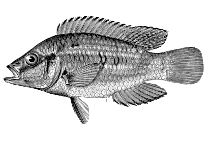
\includegraphics[width=\linewidth]{fish.png}
	\caption{An example fish.}
\end{wrapfigure}
Aliquam fringilla non diam sed varius. Suspendisse tellus felis, hendrerit non bibendum ut, adipiscing vitae diam. Lorem ipsum dolor sit amet, consectetur adipiscing elit. Nulla lobortis purus eget nisl scelerisque, commodo rhoncus lacus porta. Vestibulum vitae turpis tincidunt, varius dolor in, dictum lectus. Aenean ac ornare augue, ac facilisis purus. Sed leo lorem, molestie sit amet fermentum id, suscipit ut sem. Vestibulum orci arcu, vehicula sed tortor id, ornare dapibus lorem. Praesent aliquet iaculis lacus nec fermentum. Morbi eleifend blandit dolor, pharetra hendrerit neque ornare vel. Nulla ornare, nisl eget imperdiet ornare, libero enim interdum mi, ut lobortis quam velit bibendum nibh.

\begin{itemize}
	\item First bullet point item
	\item Second bullet point item
	\item Third bullet point item
\end{itemize}

Morbi tempor congue porta. Proin semper, leo vitae faucibus dictum, metus mauris lacinia lorem, ac congue leo felis eu turpis. Sed nec nunc pellentesque, gravida eros at, porttitor ipsum. Praesent consequat urna a lacus lobortis ultrices eget ac metus. In tempus hendrerit rhoncus. Mauris dignissim turpis id sollicitudin lacinia. Praesent libero tellus, fringilla nec ullamcorper at, ultrices id nulla. Phasellus placerat a tellus a malesuada.

\begin{enumerate}
	\item First numbered list item
	\item Second numbered list item
\end{enumerate}

%------------------------------------------------

\section*{Conclusion}

Fusce in nibh augue. Cum sociis natoque penatibus et magnis dis parturient montes, nascetur ridiculus mus. In dictum accumsan sapien, ut hendrerit nisi. Phasellus ut nulla mauris. Phasellus sagittis nec odio sed posuere. Vestibulum porttitor dolor quis suscipit bibendum. Mauris risus lectus, cursus vitae hendrerit posuere, congue ac est. Suspendisse commodo eu eros non cursus. Mauris ultrices venenatis dolor, sed aliquet odio tempor pellentesque. Duis ultricies, mauris id lobortis vulputate, tellus turpis eleifend elit, in gravida leo tortor ultricies est. Maecenas vitae ipsum at dui sodales condimentum a quis dui. Nam mi sapien, lobortis ac blandit eget, dignissim quis nunc.

Donec luctus tincidunt mauris, non ultrices ligula aliquam id. Sed varius, magna a faucibus congue, arcu tellus pellentesque nisl, vel laoreet magna eros et magna. Vivamus lobortis elit eu dignissim ultrices. Fusce erat nulla, ornare at dolor quis, rhoncus venenatis velit. Donec sed elit mi. Sed semper tellus a convallis viverra. Maecenas mi lorem, placerat sit amet sem quis, adipiscing tincidunt turpis. Cras a urna et tellus dictum eleifend. Fusce dignissim lectus risus, in bibendum tortor lacinia interdum.

\begin{table}[h] % [h] forces the table to be output where it is defined in the code (it suppresses floating)
	\caption{Example table.}
	\centering
	\begin{tabular}{l l r}
		\toprule
		\multicolumn{2}{c}{Name} \\
		\cmidrule(r){1-2}
		First Name & Last Name & Grade \\
		\midrule
		John & Doe & $7.5$ \\
		Richard & Miles & $5$ \\
		\bottomrule
	\end{tabular}
\end{table}

Fusce eleifend porttitor arcu, id accumsan elit pharetra eget. Mauris luctus velit sit amet est sodales rhoncus. Donec cursus suscipit justo, sed tristique ipsum fermentum nec. Ut tortor ex, ullamcorper varius congue in, efficitur a tellus. Vivamus ut rutrum nisi. Phasellus sit amet enim efficitur, aliquam nulla id, lacinia mauris. Quisque viverra libero ac magna maximus efficitur. Interdum et malesuada fames ac ante ipsum primis in faucibus. Vestibulum mollis eros in tellus fermentum, vitae tristique justo finibus. Sed quis vehicula nibh. Etiam nulla justo, pellentesque id sapien at, semper aliquam arcu. Integer at commodo arcu. Quisque dapibus ut lacus eget vulputate.

%----------------------------------------------------------------------------------------
%	BIBLIOGRAPHY
%----------------------------------------------------------------------------------------

\bibliographystyle{unsrt}

\bibliography{sample.bib}

%----------------------------------------------------------------------------------------

\end{document}
